\section{Media Reader Eiffage}

\begin{figure}[h]
    \centering
    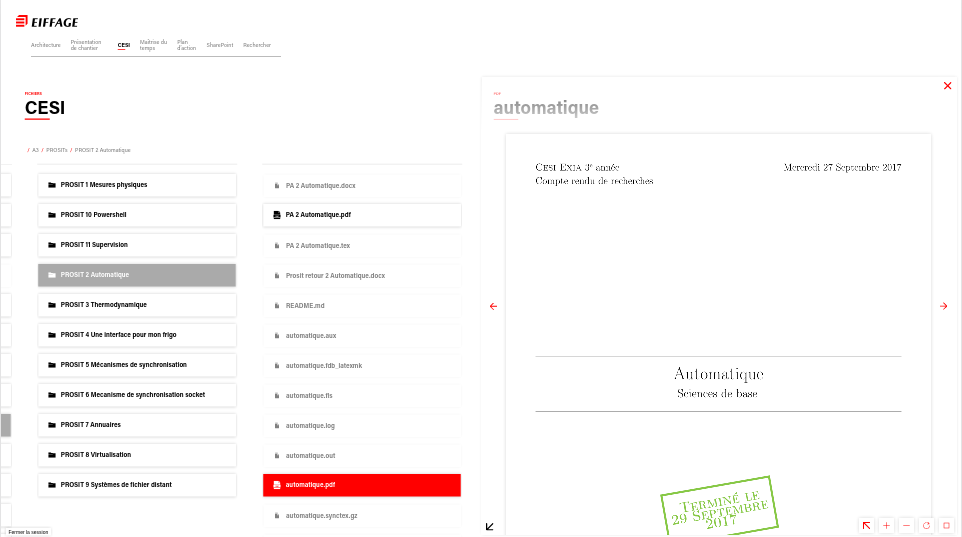
\includegraphics[scale=0.5]{img/media-reader.png}
    \caption{L'interface principale de l'application de lecture des medias Eiffage}
\end{figure}

\subsection{Eiffage}

Eiffage est un grand groupe de traveaux publics.
3\up{e} de france, il travaille sur de grands projets dans toute la france.

Dans le cadre de leur chantier de renovation Laborde, l'objectif etait de concevoir une salle de contrôle du chantier connectée.

La salle de contrôle du chantier (appelée salle cockpit) et une salle de réunion des personnes impliqués dans le déroulement du projet de rénovation.
Les plans, les problèmes et les soltions y sopnt discutés durant toute la durée du projet.
Les plans étudiés sont stockés sur un serveur central et sont disponibles aux employés pour les étudier, les annoter et les commenter.

\medskip

Nous avons mis en place 3 solutions pour ce chantier.

La première est une table tactile sur laquelle il est possible d'ouvrir, de manipuler et d'annoter les plans depuis le serveur centrale.
Cela vien remplacer les impressions successives de plans pour les annotations et les modifications.
Cela permet de réduire la consommation d'encre et de papier.

La seconde est un ecran d'affichage permettant de spitionner des Post-It sur un plan.
Ces Post-Its sont associés à une personne et définissent les tâches à accomplir.

La deniere solution est un explorateur de fichiers permettant d'afficher des photo, vidéos ou documents du chantier.
Cette solution à pour objectif de permettre un meilleur présentation du chantier avec des documents dirèctement importés depuis le serveur central.

\medskip

Dans ce projet, j'ai notemment travailler sur le navigateur de fichiers.
Ce navigateur de fichiers est affichés sur un ecran de 84 pouces tactile mettant a disposition des employés un formidable outil de présentation.

\begin{figure}[h]
    \centering
    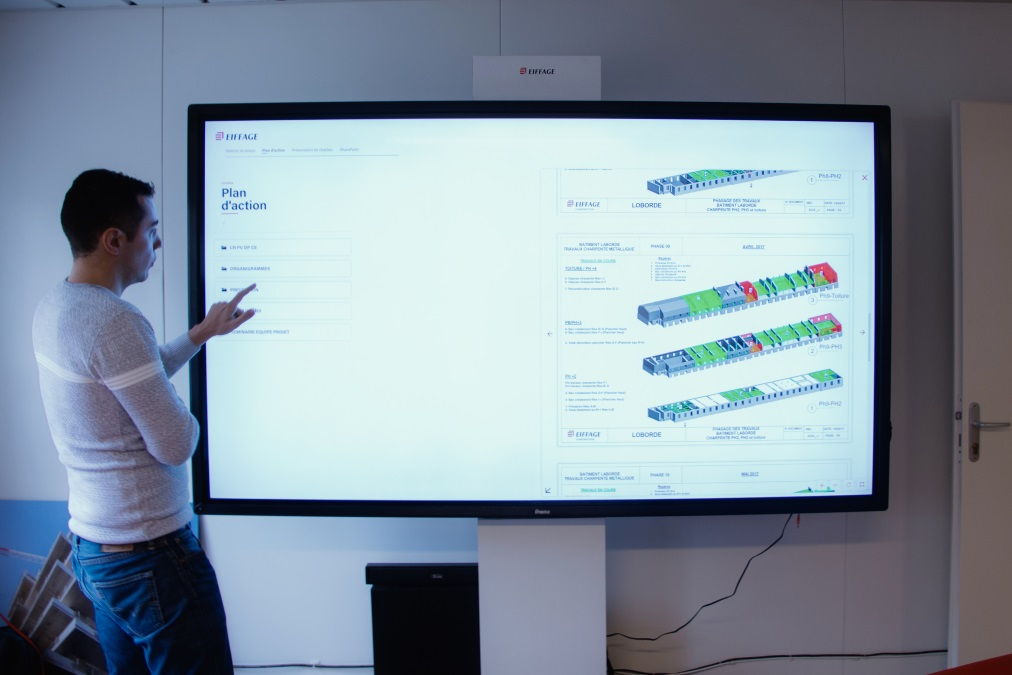
\includegraphics[scale=0.215]{img/media-reader-pres-1.jpg}
    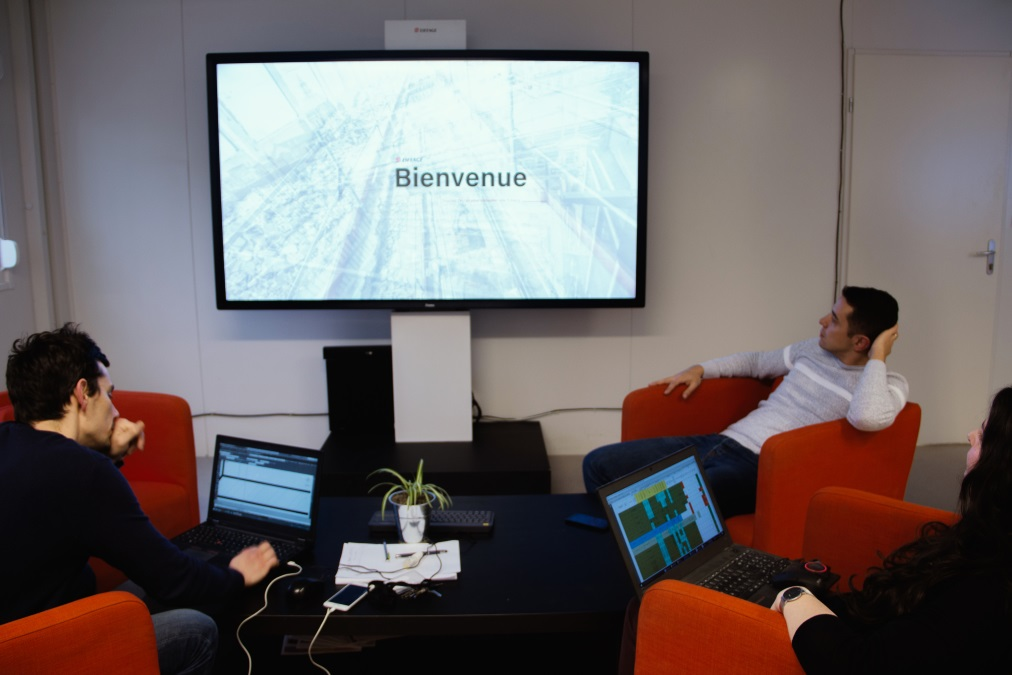
\includegraphics[scale=0.19]{img/media-reader-pres-2.jpg}
    \caption{Un aperçu de l'explorateur de fichiers une fois installé dans la salle cockpit}
\end{figure}

\subsection{Lecteur de medias}

Le lecteur de Media Eiffage doit donc disposer des fonctionnalités suivantes :

\begin{itemize}
    \item Se connecter à un emplacement réseau
    \item Lister le contenu des dossiers et pouvoir naviguer dans larborescence
    \item Afficher un aperçu des fichiers images, vidéo et PDF
    \item Integrer l'application dans un contexte Active Directory où chaque utilisateur doit pouvoir ouvrir sa session personnelle
\end{itemize}

La courte liste des fonctionnalités m'as permis de travailler plus en profondeur sur la structure de l'application et ainsi de développer des fonctionnalités solides.

\subsection{Application existante}

Due a des retard sur la livraison du materiel requis pour développer les applications Eiffage, le développement etait peu avancé.
L'explorateur de fichiers chargeait toute l'arborescense de la source des données ce qui etait peu optimisé.
En revanche la solution initial contenanit un navigateur de PDF que j'ai repris dans ma version de l'application.

Globalement, j'ai repris une grande partie de l'application qui n'utilisait pas les Webcomponents pour l'adapter aux nouvelles techniques Web permettant de modulariser chaque élément de l'interface.

\subsection{Technologies utilisés}

Pour cette application j'ai décidé d'utiliser la même technologie que les autres application de LTBL soit electron et l'utilisation des webcomponents.

Je n'ai pas utilisé de technologie supplémentaire ni de librairie complémentaire pour me former sur les futur normes web.

\subsection{Structure}

Avec ce projet, j'ai continué à expérimenter avec les webcomponents pour trouver le bon paradigme d'utilisation.
En effet, les Webcomponents présentent une structure d'application três différente des applications Web standard.
Chaque composant etant isolé des autres il faut utiliser des systèmes de communication comme les évenements javascript pour permettre une communication entre les components.

Pour ce projet j'ai fragmenté mon code sur de multiples niveaux de webcomponents.
Contrairement à l'application de BioMérieux ou j'ai fait de grand composants par grande partie de l'application.
Dans cette application, j'ai modularisé au maximum les éléments de l'interface pour pouvoir réutiliser ces composants dans un autre contexte.

\begin{figure}[h]
    \centering
    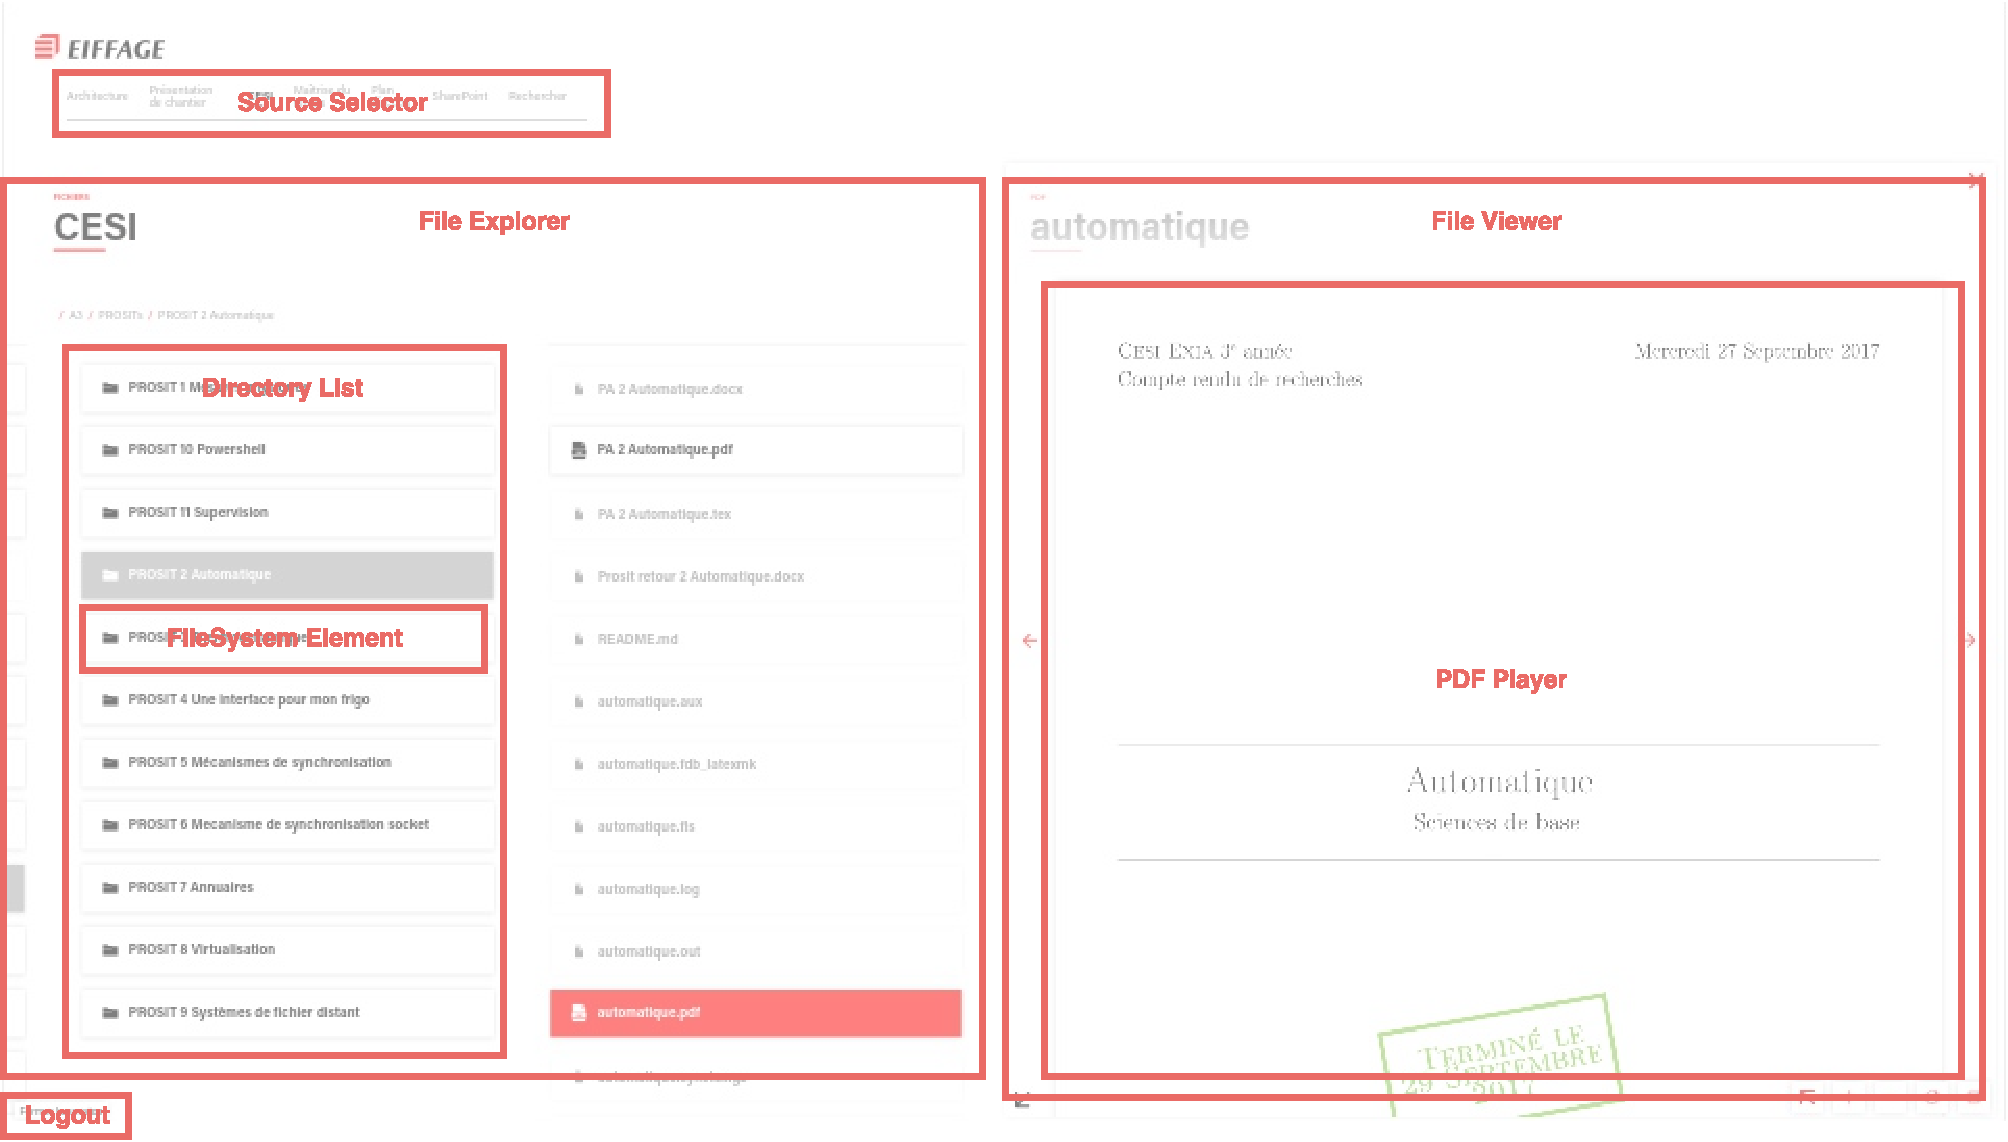
\includegraphics[scale=0.5]{img/media-reader-structure.pdf}
    \caption{La structure de l'application avec les différents components qui composent l'interface}
\end{figure}

Chaque component est séparé des autres et peux fonctionner seul sans nécéssiter d'intervention des components parents.

\begin{description}
    \item[Source Selector] Un simple menu de selectiond de selection des sources permettant a l'utilisateur de choisir parmis plusieurs elements disponibles chargés depuis un fichier de configuration général
    \item[File Explorer] Le component principal de l'application car il permet de naviguer dans les dossiers d'une source et d'ouvrir des fichiers  de cette source
    \item[Folder List] Compris dans le component \textbf{File Explorer}, il va lire le contenu d'un dossier passé en attribut et en lister le contenu
    \item[File System Element] Compris dans le component \textbf{Folder List}, ce component va chercher le fichier ou le dossier passer
    \item en attribut et afficher son titre et son icone
    \item[File Viewer] Ce component assez simple est en charge d'afficher un aperçu d'un fichier passé en attribut et de choisir le bon lecteur pour le type de fichier demandé
    \item[PDF Player] Le lecteur de fichiers, dans ce cas PDF, permettant d'afficher correctement le fichier en focntion de son type; J'ai aussi conçu \texttt{image-player} pour les images et \texttt{video-player} pour les vidéos
    \item[Logout] Un composant conçu par un collègue permettant de se deconnecter de la session windows actuelle
    \item[Lock Screen] Un component non affiché sur le schema permettant d'afficher un ecran de bienvenue avec un diaporama de photos provenant d'un emplacement réseau en arrière plan; Cet ecran de vérouillage s'affiche apres un periode d'inactivité
    \item[Web Frame] Un composant permettant d'afficher une page web avec le moteur de rendu webkit
\end{description}

\begin{figure}[h]
    \centering
    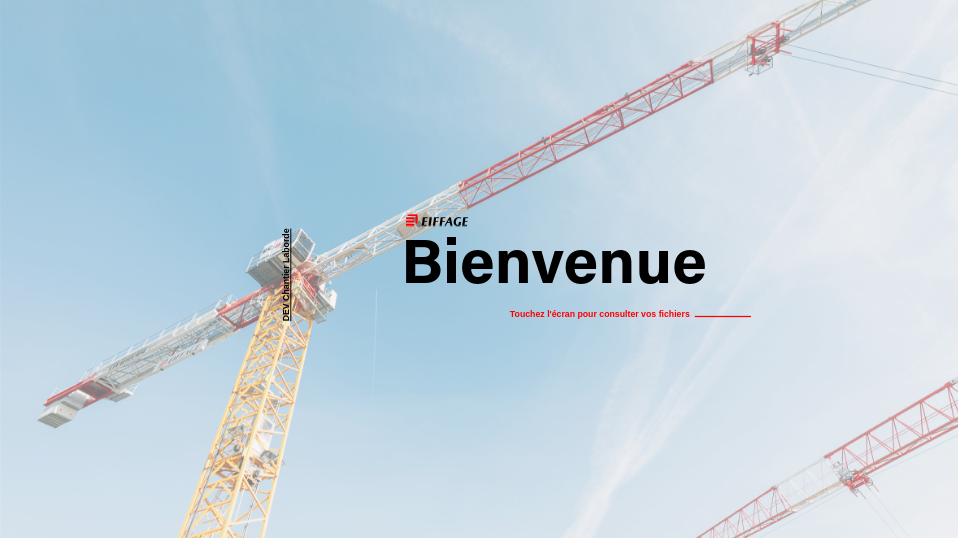
\includegraphics[scale=0.5]{img/media-reader-lock.png}
    \caption{Vue de l'ecran de vérouillage du lecteur de medias}
\end{figure}

\clearpage

\subsection{Component d'animation}

Les animation prennnent un grande place dans le design des applications de LTBL et celles-ci sont prises très au serieux par l'équipe de développement.
Les animations dans les technologies Web posent quand même un problème.
Elles doivent êtres prises en compte des la creation des éléments pour être correctement utilisables.
De plus l'animation des plusieurs éléments les uns a la suide des autres est difficile en css.

J'ai donc crée un component web en charge de gèrer les animations.
Ce component commé \texttt{Animated Block} permet de ne pas penser à l'animation pendant le développement mais de l'ajouter à la fin, des que les fonctionnalités sont ajoutés comme une dernière finition.
Ce component propose un système d'animation se basant sur les transitions CSS (bien plus performantes que les animations JavaScript) et les classes des element à animer.

L'\texttt{Animated Block} se présente comme un bloc transparent, qui n'a pas d'incidence sur le style global de l'application.
Il régis comme un \texttt{div} et paut facilement remplacer un élément de l'interface pour l'animer.

Un \texttt{Animated Block} propose 2 animations par défaut \texttt{enter} et \texttt{leave} servant respectivement a faire apparaitre l'élément et a le faire disparaitre.
Le component n'impose pas d'animation de base mais met à disposition système permettant de faire une animation facilement.

Par exemple, prenons l'animation \texttt{enter}.

\begin{figure}[h]
    \centering
    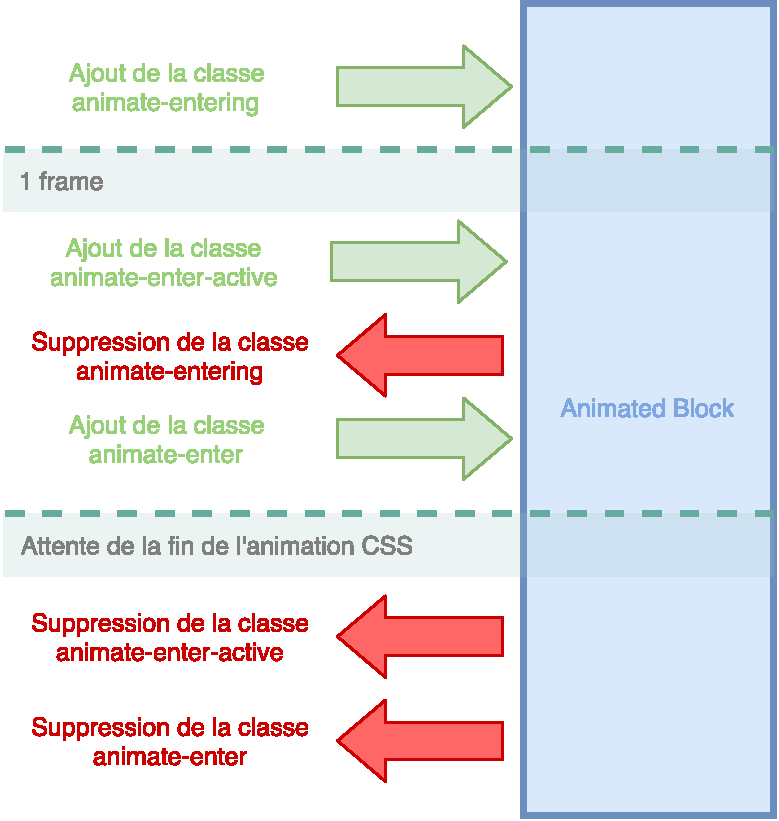
\includegraphics[scale=0.5]{img/animated-block.pdf}
    \caption{Système d'animation d'\texttt{Animated Block}}
\end{figure}

Chaque animation est composée de 3 classes permettant de créer le movement correct

\begin{description}
    \item[Classe de setup] En charge de mettre en style l'élément avant l'animation (Ex. placer l'élément hors de l'ecran pour le faire apparaitre)
    \item[Classe d'animation] Gèrant l'animation dans son ensemble, c'est sur cette classe que l'on positionne la propriété de \texttt{transition} css permettant d'animer les différents styles de bloc
    \item[Classe d'etat final] En charge de définir l'etat final de l'élément apres l'animation (Elle n'est pas necessaire si l'etat final est le même que l'etat standard du bloc)
\end{description}

Ainsi, tout l'animation passe par le fait d'ajouter ou de retirer ces classes.
Le pipeline d'animation est alors le suivant :

\begin{enumerate}
    \item On ajoute la classe de setup (\texttt{animate-entering} dans notre cas)
    \item Une frame plus tard (une fois l'élément stylisé) on ajoute la classe d'animation (\texttt{animate-enter-active} dans notre cas)
    \item On retire la classe de setup puis on ajoute la classe d'etat final (\texttt{animate-enter} dans notre cas)
    \item On calcul le temps de l'animation puis on attend la fin de celle-ci
    \item On retire la classe d'animation et d'etat final
\end{enumerate}

Il est bien sur possible de créer ses propres animations en spécifiant manuellement les différentes classes à utiliser mais les deux animations (\texttt{enter} et \texttt{leave}) sont des animations normalisés.

Des qu'une animation est déclenchée, une promesse est renvoyée pour permettre de savoir suand elle se treminera.
Cela permet d'éfféctuer des actions apres que l'annimation soit passée comme réinitialiser des données ou éfféctuer des action en arrière plan.

Enfin, le component \texttt{Animated Block} dispose d'une fonction statique \texttt{animateStack()} permettant d'animer un ensemble d'éléments les uns apres les autres en éxécutant simplement une fonction.

Ainsi, grâce a ce système, on peux simplement ajouter des animations au projet sans ajouter beaucoup de lignes de code pouvant mener à des bugs.
Il suffit d'appeler la fonction d'annimation et d'attendre la résolution de la promesse pour éfféstuer des actions apres l'animation.